\section{Einleitung}
Wenn Kräfte $F_{\symup{i}}$ auf einen Körper wirken, kann es bei hinreichender Kraft zu einer Deformierung des Körpers kommen.
Das Elastizitätsmodul $E$ ist eine Kenngröße dieser Deformation und wird in diesem Versuch für zwei Körper aus Kupfer bestimmt.

\section{Theorie}
\label{sec:Theorie}

\subsection{Das Hooksche Gesetz}
\label{sec:hook}
In dem Fall, dass eine auf einen Körper wirkende Spannung eine hinreichend kleine Änderung einer Körperdimension 
$\frac{\Delta L}{L}$ bewirkt, besteht ein linearer Zusammenhang zwischen der Spannung, der durch das 
\textit{Hooksche Gesetz}(\autoref{eq:hook}) beschrieben wird. Der Proportionalitätsfaktor $E$ wird als Elastizitätsmodul 
definiert und ist eine material- und formabhängige Konstante.
\begin{equation}
    \sigma = E \cdot \frac{\Delta L} {L} \notag
    \label{eq:hook}
\end{equation}

\subsection{Durchbiegung eines Stabes bei einseitiger Einspannung}
\label{sec:einseitig}
Wird ein Stab, wie in \autoref{fig:stab einseitig eingespannt} zu sehen, einseitig eingespannt, verbiegt er sich bereits 
unter seinem Eigengewicht. An jeder Stelle $x$ des Stabes kann eine Durchbiegung $D(x)$ festgestellt werden.
Wird weiteres Gewicht an ein Stabende angehängt, wirkt eine größere Gewichtskraft $F_{\symup{G}}$ und der Stab 
verbiegt sich stärker, die Durchbiegung $D(x)$ wird an jeder Stelle $x$ größer.
\begin{figure}
    \centering
    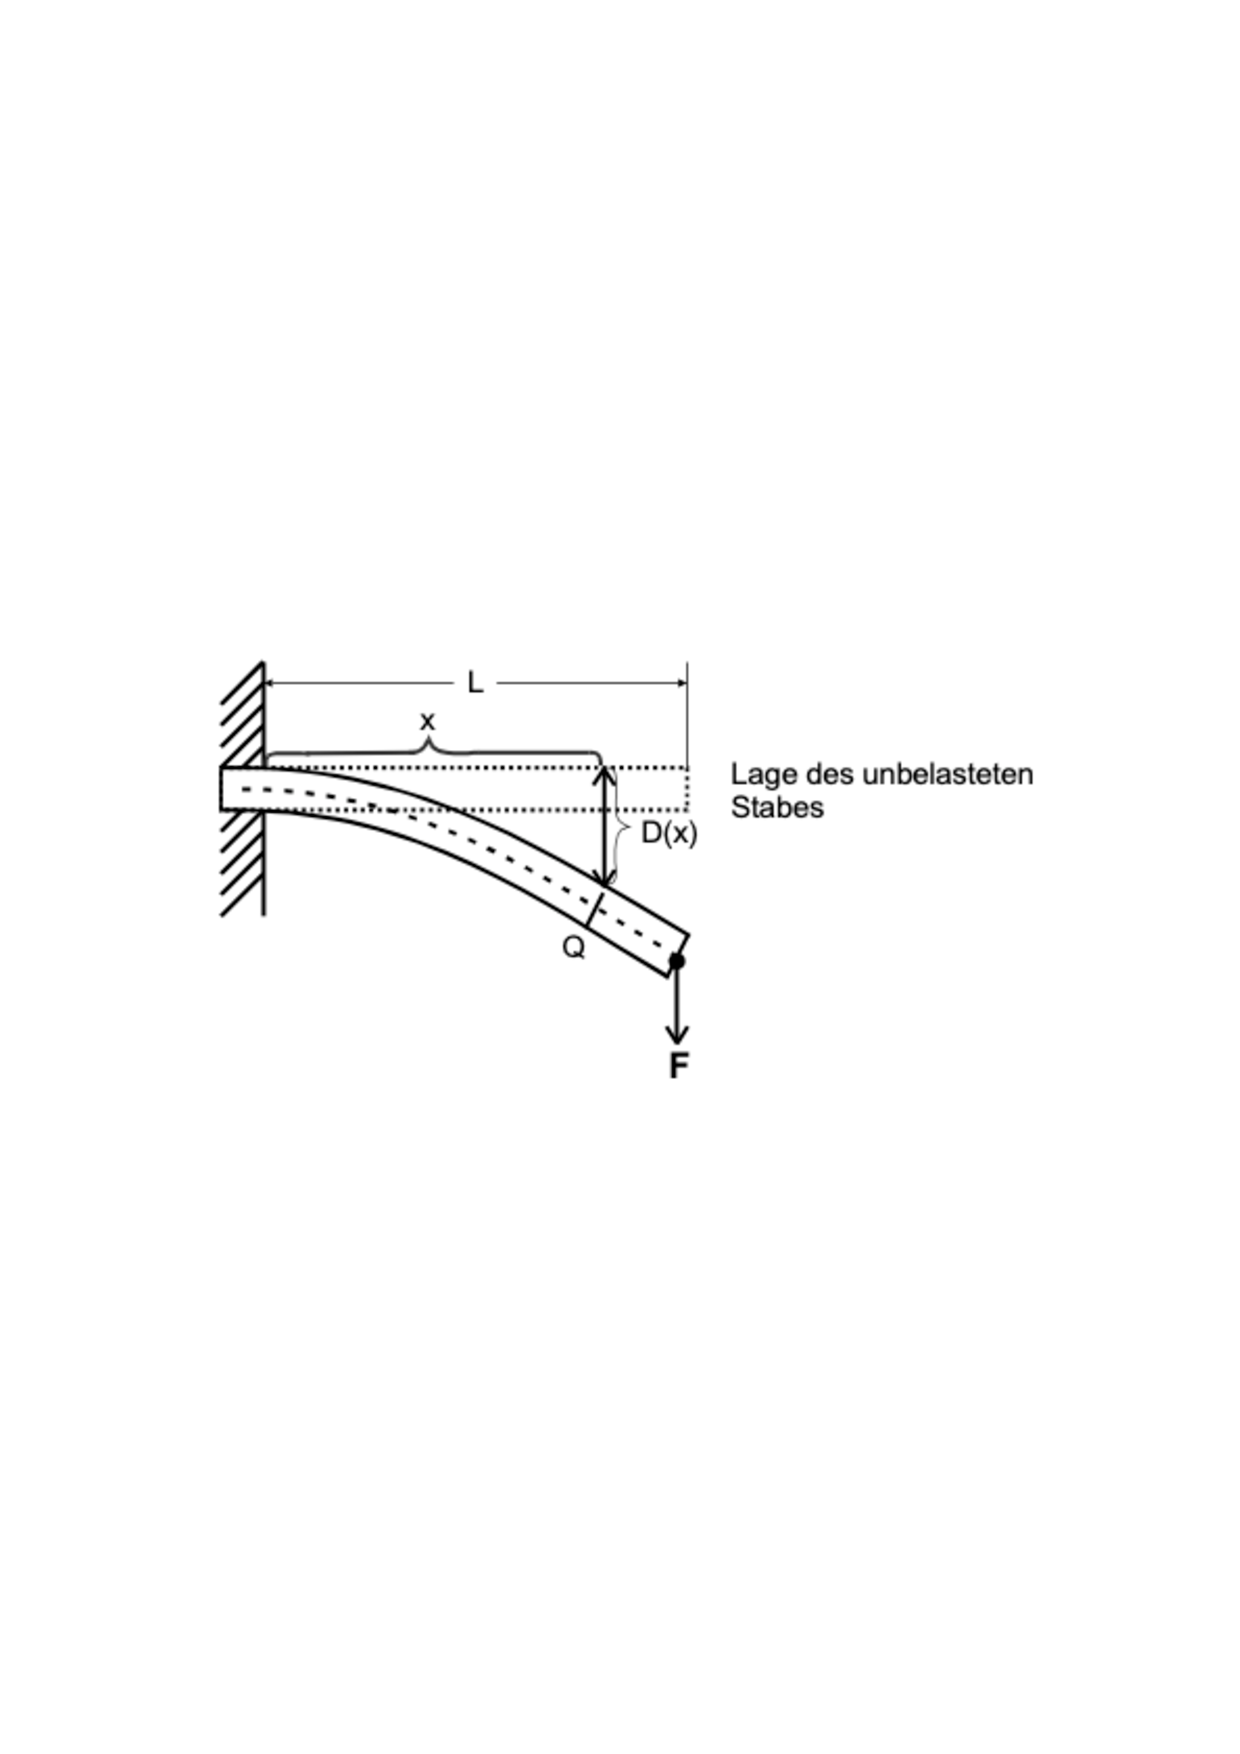
\includegraphics[height=6cm]{content/Abbildungen/stab_einseitig_eingespannt.pdf}
    \caption{Einseitig eingespannter Stab. \cite{v103}}
    \label{fig:stab einseitig eingespannt}
\end{figure}

Die wirkende Gewichtskraft $F_{\symup{G}}$ hat zur Folge, dass in dem Stab Drehmomente $M$ wirken, die den Stab aus seiner 
Ruhelage verdrehen. Diesen Drehmomente $M$ gegenüber treten Normalenspannungen auf und es stellt sich ein 
Gleichgewichtszustand mit endgültiger Durchbiegung $D(x)$ ein. Der obere Teil wird durch vorhandene Zugspannungen 
gestreckt während der untere Teil durch Druckspannungen gestaucht wird. Zwischen diesen Teilen liegt eine Fläche, die 
ihre ursprüngliche Länge beibehält und als \textit{neutrale Phase} bezeichnet wird. Die Zug- und Druckspannungen $\sigma$, 
welche an der neutralen Phase angereifen, sind genau entgegengesetzt und heben sich daher auf. 
Die \autoref{fig:neutrale phase} verdeutlicht dies.

\begin{figure} [H]
    \centering
    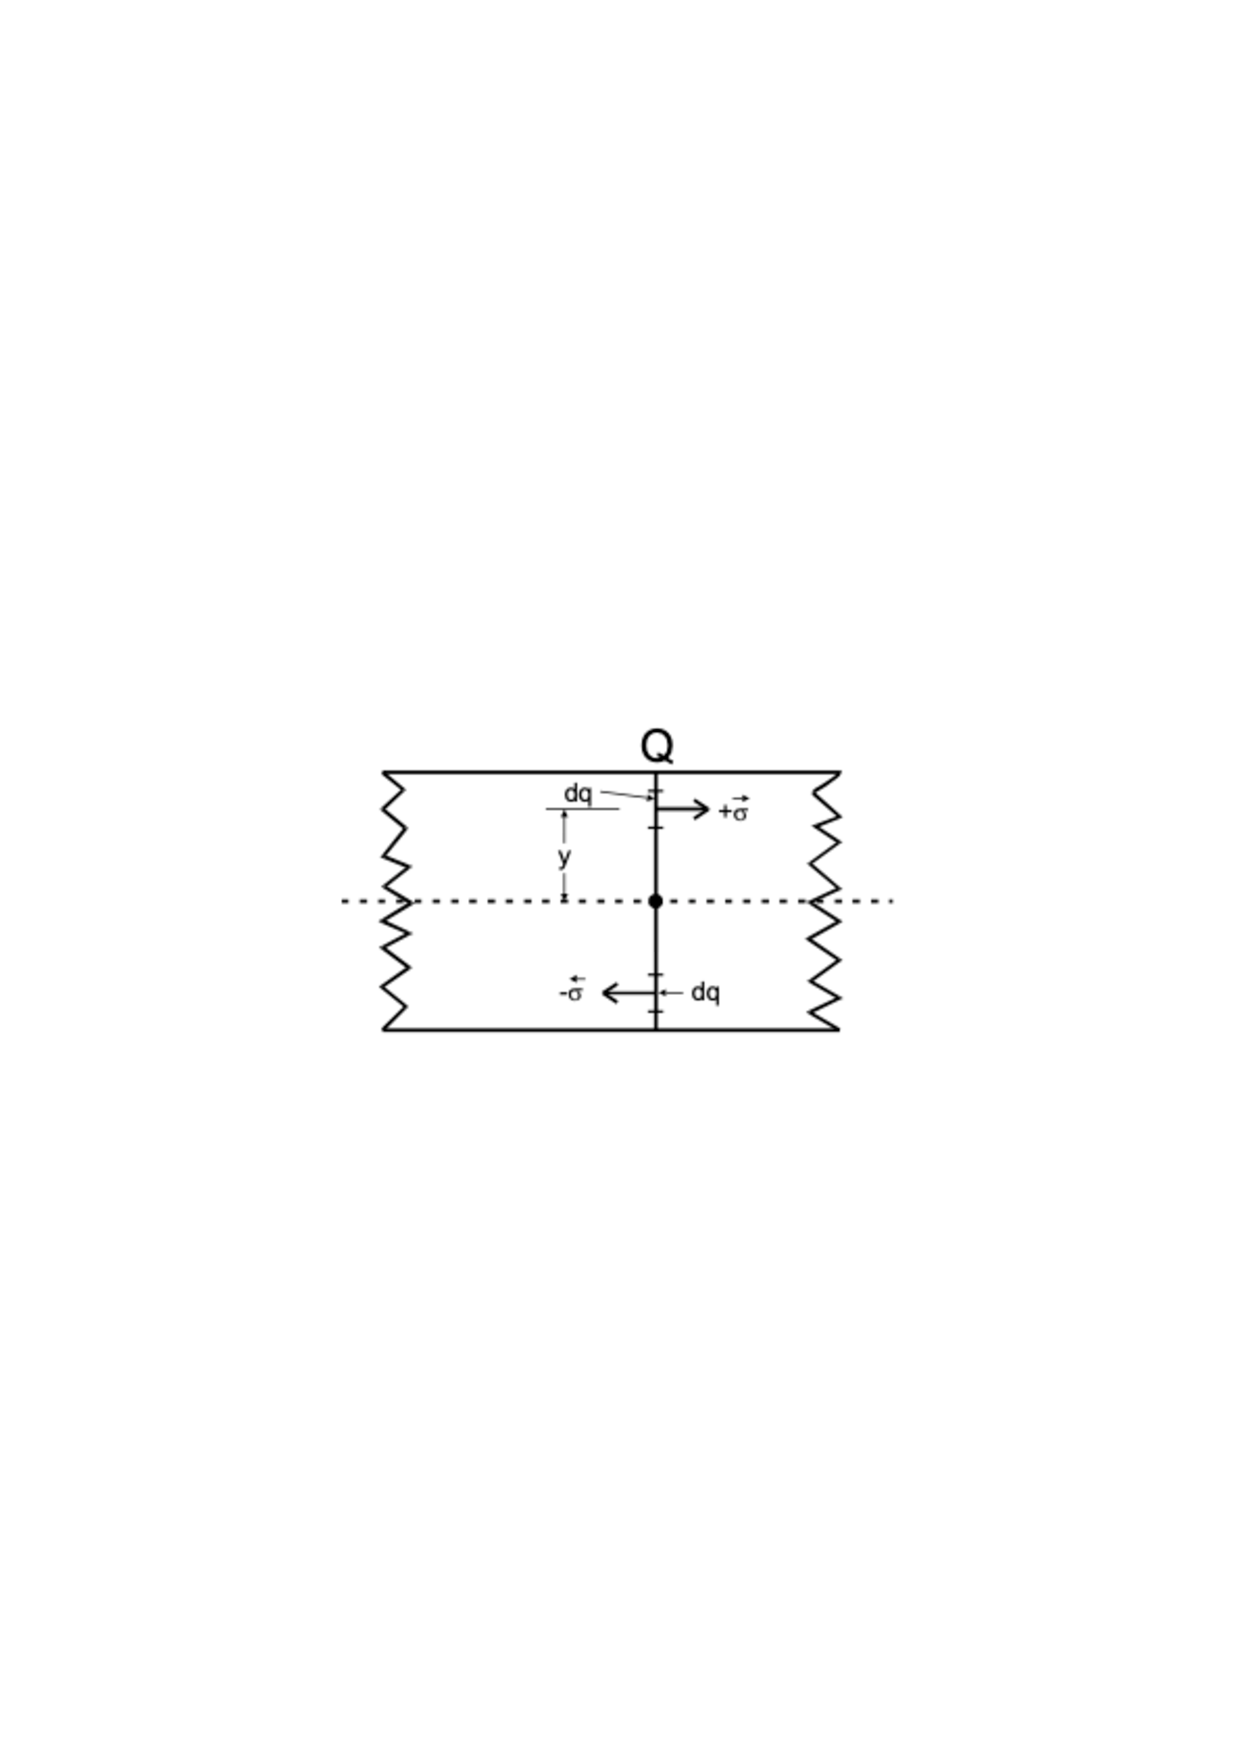
\includegraphics[height=6cm]{content/Abbildungen/neutrale_phase.pdf}
    \caption{Neutrale Phase mit wirkenden Zug- und Druckspannungen $\sigma$. \cite{v103}}
    \label{fig:neutrale phase}
\end{figure}

% Das an der neutralen Phase $Q$ wirkende Drehmoment lässt sich also schreiben als:
% \begin{equation}
%     M_{\symup{\sigma}}=\int_{Q}y\sigma(y)\symup{d}q
%     \label{eq:drehmoment neutrale phase}
% \end{equation}
% Hierbei bezeichnet $y$ den Abstand des Flächenelements d$q$ von der neutralen Phase $x$ und $Q$ einen Querschnitt des Körpers.

% HIER FEHLT NOCH ETWAS HERLEITUNG %%%%%%%%%%%%%%%%%%%%%%%%%%%%%%
Für die Durchbiegung $D(x)$ lässt sich eine Formel aufstellen, wobei $x=0$ den eingespannten Punkt
und $x=L$ den Endpunkt des Stabes beschreibt:

\begin{equation}
    D(x)=\frac{F}{2EI}(Lx^{2}-\frac{1}{3}x^{3})
    \label{eq:Durchbiegung einseitig}
\end{equation}

Dabei beschreibt $F$ die Gewichskraft, $E$ das Elastizitätsmodul und $I$ das Flächenträgheitsmoment.
Für einen runden Stab ist $I$ gegeben durch:

\begin{equation}
    I=\frac{\pi}{4}R^{4}
    \label{eq:Flächenträgheitsmoment rund}
\end{equation}

\subsection{Durchbiegung eines Stabes bei zweiseitiger Auflage}
\label{sec:zweiseitig}

Nun wird der Stab wieder mit einem Gewicht belastet, welches hier jedoch in dessen Mitte platziert wird.
Die Enden des Stabes liegen dabei nur auf und sind nicht wie in \autoref{sec:einseitig} fest eingespannt,
\autoref{fig:stab beidseitig} verdeutlicht dies.

\begin{figure} [H]
    \centering
    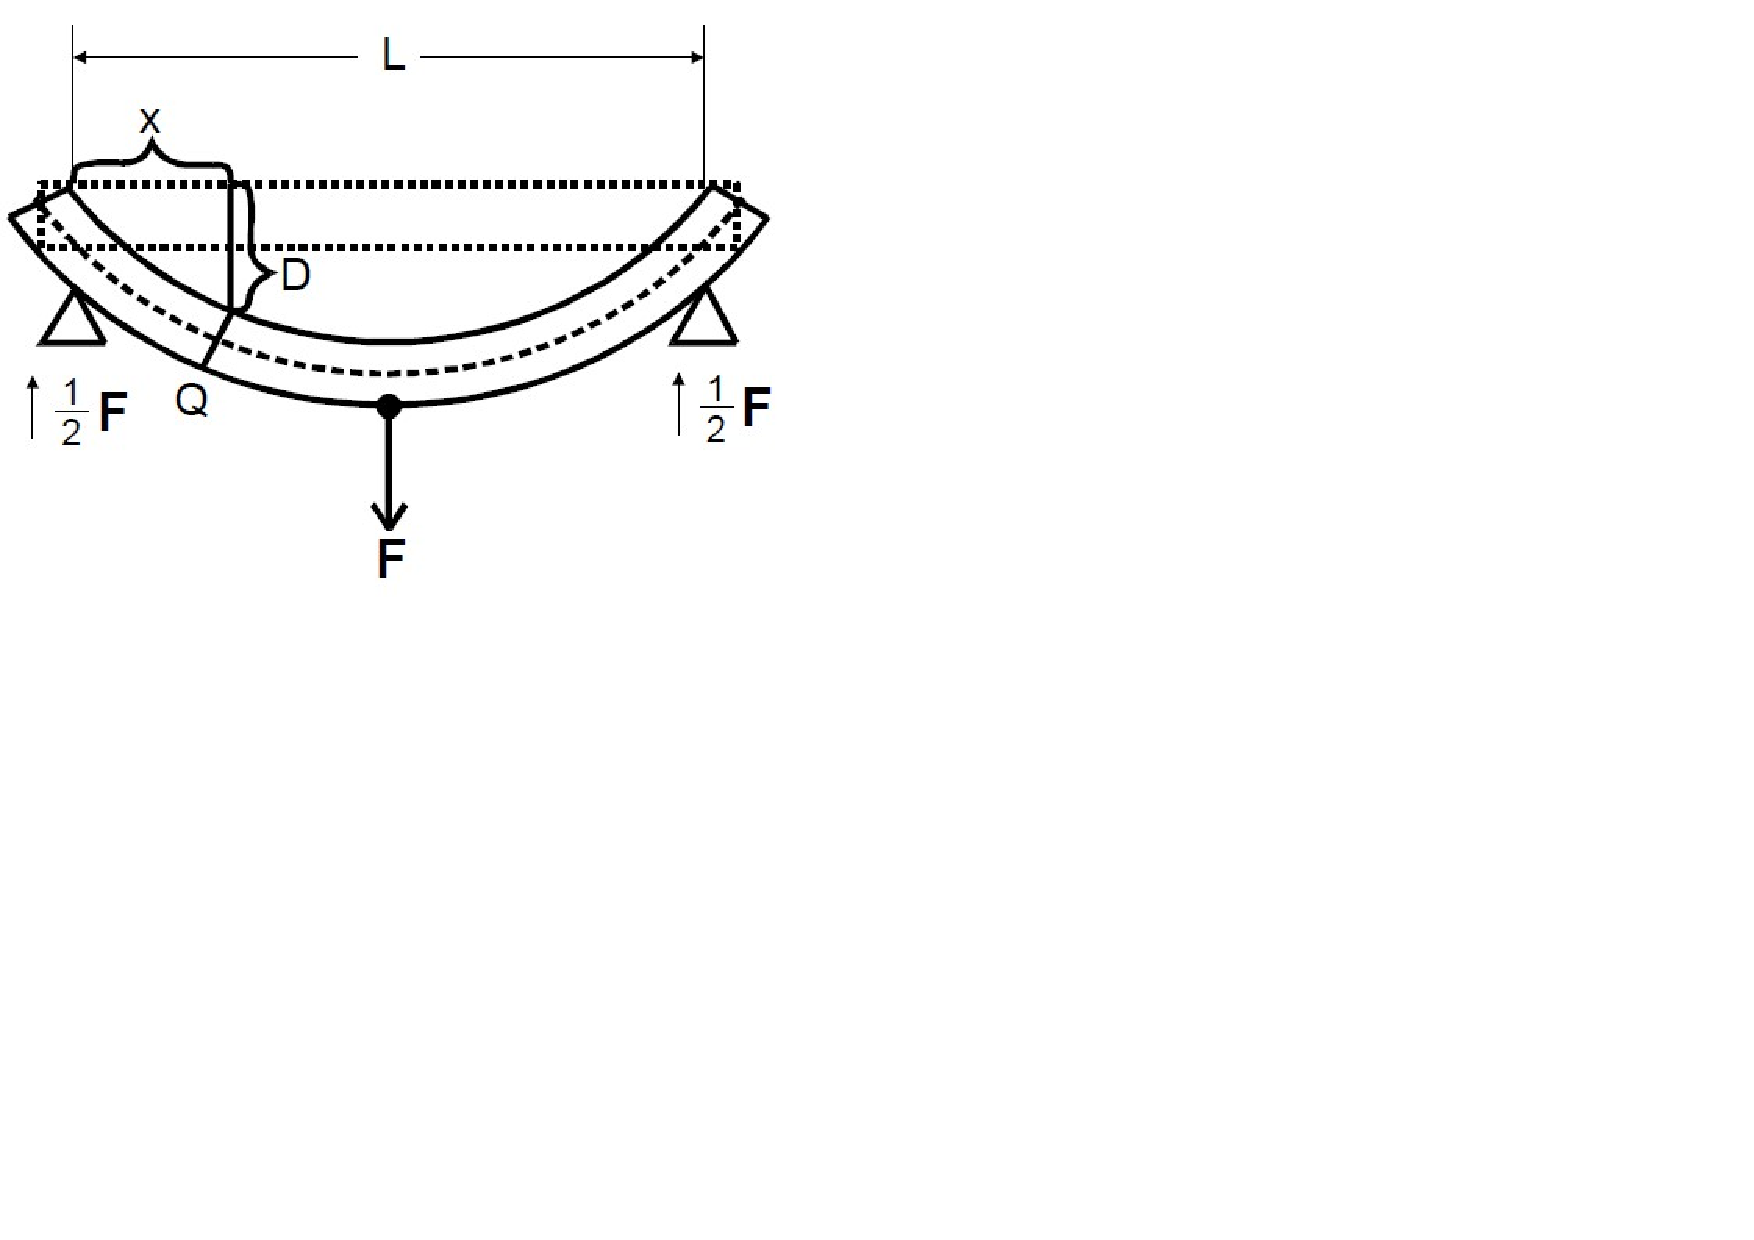
\includegraphics[height=6cm]{content/Abbildungen/stab_beidseitig.pdf}
    \caption{Beidseitig aufliegender Stab. \cite{v103}}
    \label{fig:stab beidseitig}
\end{figure}

Für die Durchbiegung $D(x)$ erhält man nun 2 Formlen, abhängig von der Position auf dem Stab.
Für $0\leq x\leq \frac{L}{2}$ gilt:

\begin{equation}
    D(x)=\frac{F}{48EI}(3L^{2}x-4x^{3})
    \label{eq:Durchbiegung beidseitig 1}
\end{equation}

Und für $\frac{L}{2}\leq x\leq L$ ergibt sich:

\begin{equation}
    D(x)=\frac{F}{48EI}(4x^{3}-12Lx^{2}+9L^{2}x-L^{3})
    \label{eq:Durchbiegung beidseitig 2}
\end{equation}

Für einen eckigen Stab mit quadratischem Querschnitt der Kantenlänge $a$ bestimmt sich das Flächenträgheitsmoment $I$ zu: 

\begin{equation}
    I=\frac{1}{12}a^{4}
    \label{eq:Flächenträgheitsmoment eckig}
\end{equation}

\subsection{Versuchsapparatur}
\label{sec:Apparatur}

Um die Durchbiegung genau zu messen, wird die in \autoref{fig:Apparatur} abgebildete Apparatur verwendet.
Die Stäbe können damit einseitig eingespannt oder beidseitig aufgelegt werden.
Darüber befinden sich auf einer Schiene zwei Messuhren, mit denen der Abstand zum Stab präzise gemessen werden kann.

\begin{figure} [H]
    \centering
    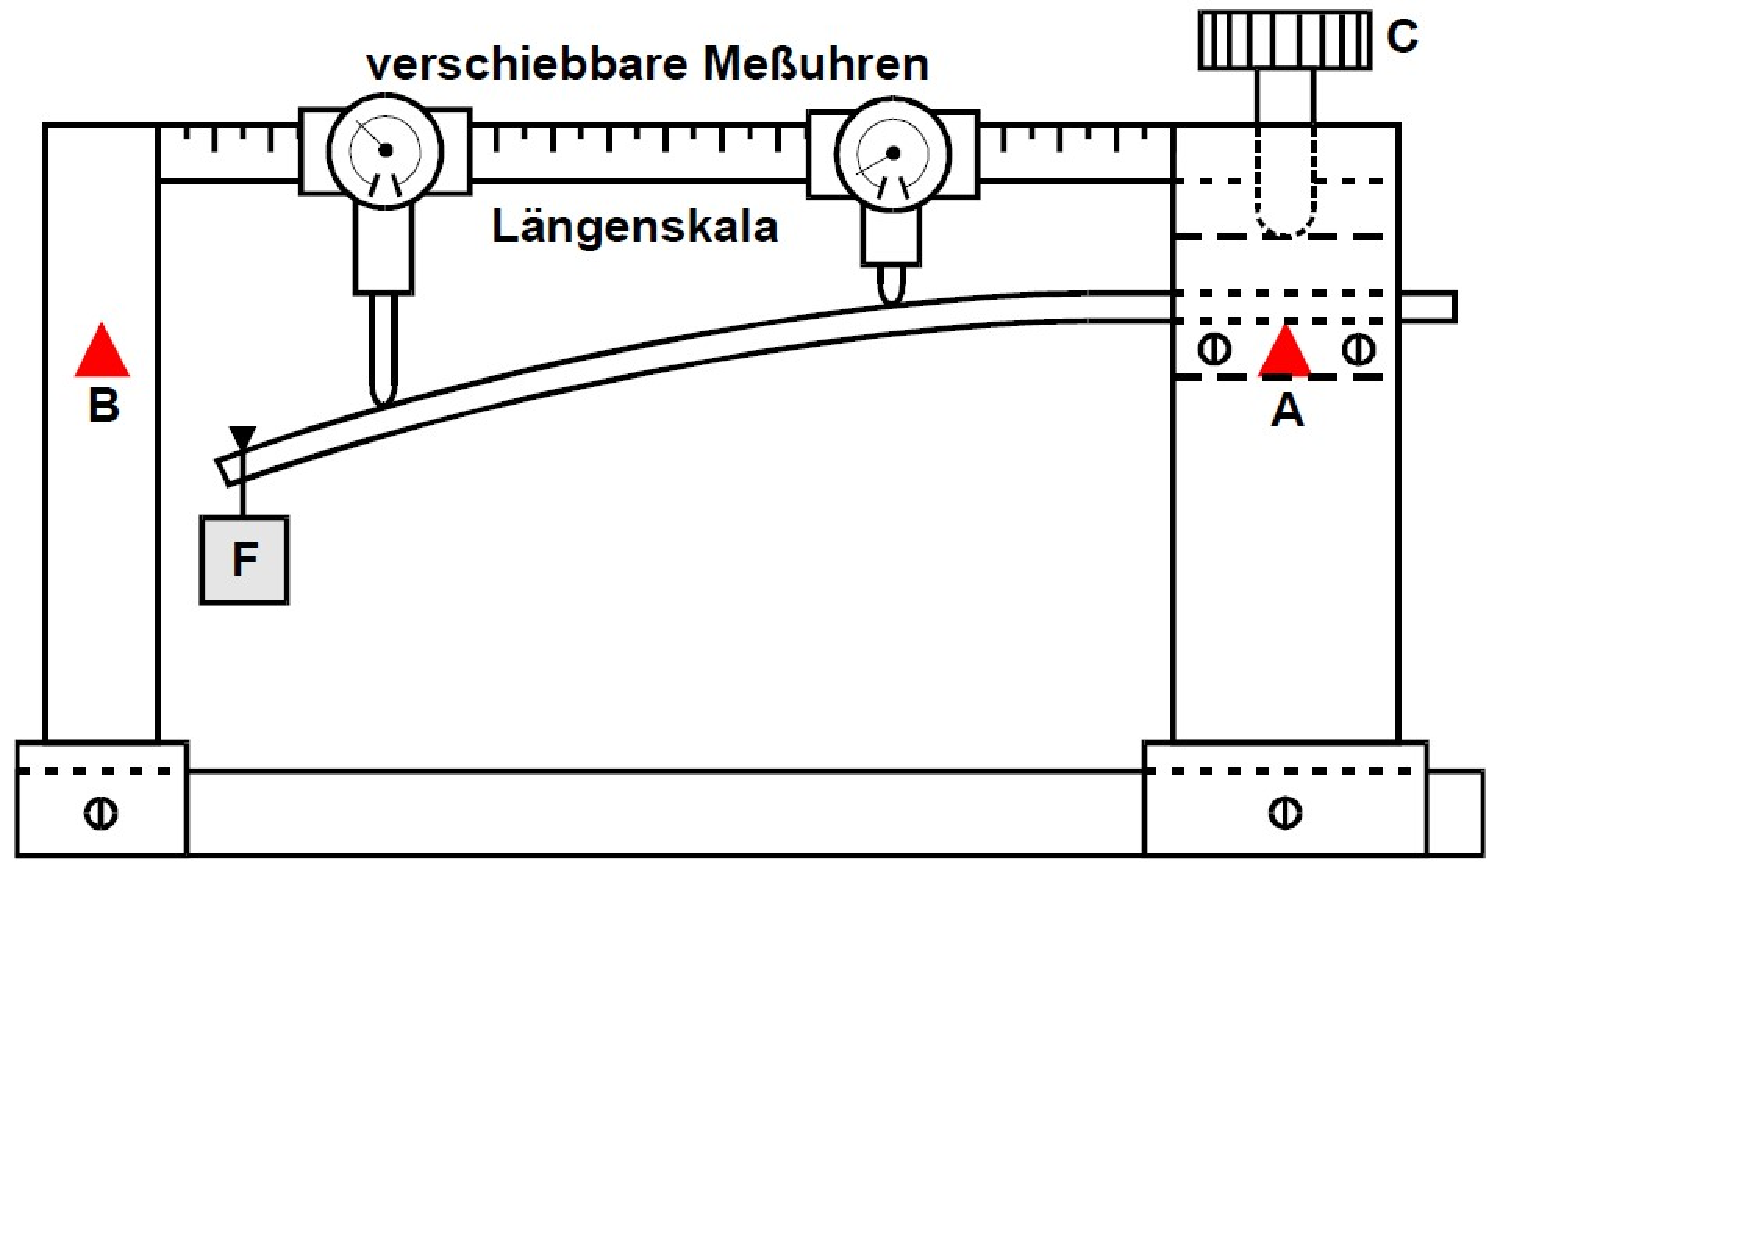
\includegraphics[height=6cm]{content/Abbildungen/Apparatur.pdf}
    \caption{Versuchsapparatur. \cite{v103}}
    \label{fig:Apparatur}
\end{figure}